A partir de la gráfica de la figura \ref{fig:SINMAT1_U3_AC75_IMG3} que registra el cambio de temperatura con respecto al tiempo, de una muestra de agua a la que se aplica una cantidad constante de calor, escribe la cantidad correcta en el cuadro de texto.
\begin{figure}[H]
    \centering
    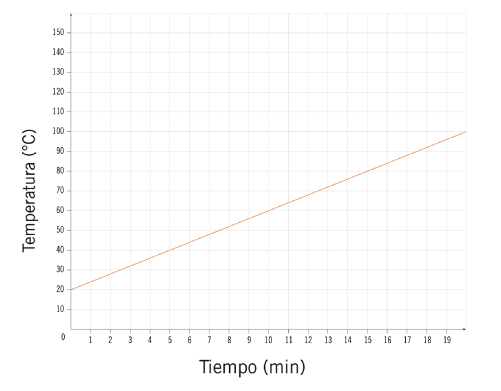
\includegraphics[width=0.75\textwidth]{../images/SINMAT1_U3_AC75_IMG3.jpg}
    \caption{Tabla de precios de los direrentes reciclables.}
    \label{fig:SINMAT1_U3_AC75_IMG3}
\end{figure}
\begin{parts}
    \include*{../parts/question075c01}
    \include*{../parts/question075c02}
    \include*{../parts/question075c03}
    \include*{../parts/question075c04}
    \include*{../parts/question075c05}

\end{parts}